%!TEX root = ../crimson_throne_book_main.tex
% 2013-05-19
The last thing Balian remembered of his father were the words {\itshape ``Run, son, run, and take your sister!''}. That was two and a half years ago, when he used to live in the North Point District.\\

Back in the day Balian's father ran a simple second hand store, trying to make enough money to feed his two children, his eleven year old son and a nine year old daughter, Alika. Still, life was hard for the widower, who sometimes fenced stolen goods from a local thug, Gaedran Lamm, to make ends meet. This welcome addition to his income would be his undoing, for when an unsuspecting customer recognized her stolen bracelet, she warned the Korvosan Guard. The next day the guards busted the shop to confront the shopkeeper and arrest him and his son, but the desperate man pushed his boy aside and urged him to take his sister and run. Meanwhile he tried to hold off the guards, knocking over a lantern in the struggle. The building caught fire and the poor shopkeeper perished in the flames.\\

A couple of days later, while Balian and his sister were wandering aimlessly through the streets of Korvosa, they came across a creepy, old man. He introduced himself as Gaedran Lamm and told them that a number of his goods had been in their father's shop when it had burnt down. Things that hadn't been paid for yet. Korvosan law and custom dictated that a man's debts were inherited by his heirs, so the children now owed a debt to Lamm. To settle the score Balian and Alika would have to work for Lamm for free until the man decided that the money was repaid. If the children refused, he threatened to call the guard and have the little fugitives arrested. Moreover, he wouldn't hesitate to harm any one of them of the other was too much trouble.\\

Ever since that time Balian has been one of Lamm's lambs, a gang of child slave laborers and pickpockets. His master never lets him forget that he ``owes'' him, and regularly gives him a firm beating, sometimes even without apparent cause. Since he fears for his sister's safety, the boy tries to avoid doing anything wrong.\\

Luckily, he's made some new friends among his fellow lambs, most notably Sjo, a tall boy of Shoanti blood, and Quint, a clear-eyed youngster of Chelish stock. Both boys have been with Lamm for as long as they can remember and have never known anything but hardship. All Sjo has to remind him of his origin is a weathered wooden board with his name in Shoanti runes, ``Shaoban'', which quickly wore down to ``Sjo''. Quint lacks even that, although he has a rather distinguishable birthmark on his shoulder that resembles a curled-up scorpion. Lamm refers to this spot as the "devil's touch'', and fears the boy because of it. He doesn't beat the boy as often as the others and his punishments are rarely as severe.\\

%!TEX root = ../crimson_throne_book_main.tex
\section{Level 0 (Children)}
\def\h{0.4}
\begin{center}
\resizebox{!}{\h\textheight}{
    %%%%%%%%%%%%%%%%%%%%%%%%%%%%%%%%%%%%%%%%%%%%%%%%%%%%
    %%% SHAOBAN
    %%%%%%%%%%%%%%%%%%%%%%%%%%%%%%%%%%%%%%%%%%%%%%%%%%%%
	\begin{tikzpicture}[font=\footnotesize,node distance=0em]
		% Frame
		\fill[yellow!10, draw=black, rounded corners] ($(0,0) + (-0.25cm,0.25cm)$) rectangle (8cm,-12cm);	
	
		\node[below right] at (8cm-2cm-0.25cm-0.25cm,0) {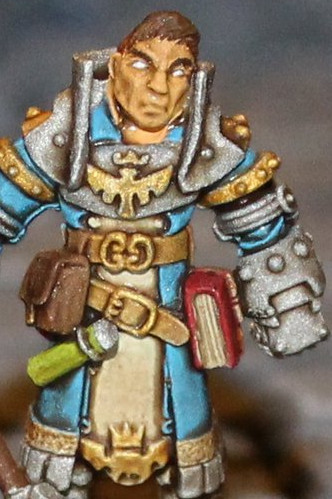
\includegraphics[width=2cm, height=3cm]{C:/privat/rpg/crimson_throne_book/latex/images/shaoban}};
	
		\node[below right,font=\bfseries\setmainfont{Immortal}\large] (name) at (0,0) {SHAOBAN};

		\node[below=of name.south west,below right,yshift=0.5em] (info){LN small human};
		
		\node[below=of info.south west,below right, align=left] (skills) {
                Init +0; Senses Perception +2\\ 
                Common
		};

		\node[below=of skills.south west,below right, align=left] (ac){
                AC 11, touch 11, flat-footed 11\\
                HP 5 (1HD)\\
                Fort -1, Ref +0, Will +2
		};
	

		\node[below=of ac.south west,below right, align=left] (fight) {
                Speed 30 ft. (6 squares)\\
                Melee dagger (small) +1 (1d3/19-20)\\
                Ranged dagger (small/thrown) +1 (1d3/19-20)\\
                Face 5 ft. Reach 5 ft.\\
                Base Atk +0; CMB -1; CMD 9
        };

		\node[below=of fight.south west,below right, align=left] (abilities) {
                Str 10, Dex 10, Con 8, Int 8, Wis 14, Cha 18
	   };

		\node[below=of abilities.south west,below right, align=left] (feats) {
                Simple Weapon Proficiency
	   };

		\node[below=of feats.south west,below right, align=left, text width=7.5cm] (skills) {
            Appraise -1, Bluff +4, Diplomacy +7, Disguise +4,\\ 
            Fly +2, Heal +2, Intimidate +5, Perception +2,\\ 
            Sense Motive +6, Sleight of Hand +6, Stealth +4,\\ 
            Survival +2
	   };

		\node[below=of skills.south west,below right, align=left, text width=7.5cm] (poss) {
            Dagger (small) 
	   };
	
		\node[below=of poss.south west,below right, align=left, text width=7.5cm] (traits) {
            {\itshape Child of the Streets:} {\scriptsize You grew up on the streets of a large city, and as a result you have developed a knack for picking pockets and hiding small objects on your person. You gain a +1 trait bonus on Sleight of Hand checks, and Sleight of Hand is always a class skill for you.}\\
            {\itshape Ease of Faith:} {\scriptsize  Your mentor, the person who invested your faith in you from an early age, took steps to ensure that you understood that what powers your divine magic is no different than that which powers the magic of other religions. You gain a +1 trait bonus on Diplomacy checks, and Diplomacy is always a class skill for you.}
        };
	\end{tikzpicture}
    \hspace{1cm}
    %%%%%%%%%%%%%%%%%%%%%%%%%%%%%%%%%%%%%%%%%%%%%%%%%%%%
    %%% Quintilian
    %%%%%%%%%%%%%%%%%%%%%%%%%%%%%%%%%%%%%%%%%%%%%%%%%%%%
	\begin{tikzpicture}[font=\footnotesize,node distance=0em]
		% Frame
		\fill[yellow!10, draw=black, rounded corners] ($(0,0) + (-0.25cm,0.25cm)$) rectangle (8cm,-12cm); 
    
        \node[below right] at (8cm-2cm-0.25cm-0.25cm,0) {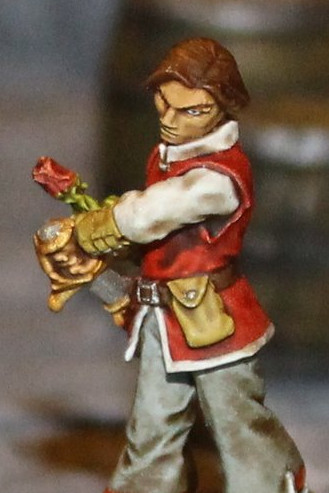
\includegraphics[width=2cm, height=3cm]{C:/privat/rpg/crimson_throne_book/latex/images/quint}};
    
        \node[below right,font=\bfseries\setmainfont{Immortal}\large] (name) at (0,0) {QUINTILIAN};

        \node[below=of name.south west,below right,yshift=0.5em] (info){CG small human};
        
        \node[below=of info.south west,below right, align=left] (skills) {
                Init +2; Senses Perception -1\\ 
                Common
        };

        \node[below=of skills.south west,below right, align=left] (ac){
                AC 13, touch 13, flat-footed 11\\
                HP 5 (1HD)\\
                Fort -1, Ref +2, Will -1
        };
    

        \node[below=of ac.south west,below right, align=left] (fight) {
                Speed 30 ft. (6 squares)\\
                Melee dagger (small) +1 (1d3/19-20)\\
                Ranged dagger (small/thrown) +1 (1d3/19-20)\\
                Face 5 ft. Reach 5 ft.\\
                Base Atk +0; CMB -1; CMD 11
        };

        \node[below=of fight.south west,below right, align=left] (abilities) {
                Str 10, Dex 14, Con 8, Int 14, Wis 8, Cha 16
       };
	\end{tikzpicture}
}

\resizebox{!}{\h\textheight}{
	\begin{tikzpicture}
		% Frame
		\fill[yellow!10, draw=black, rounded corners] ($(0,0) + (-0.25cm,0.25cm)$) rectangle (8cm,-12cm);	
	
		\node[below right] at (8cm-2cm-0.25cm-0.25cm,0) {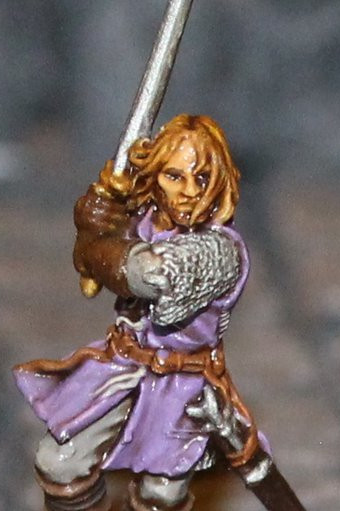
\includegraphics[width=2cm, height=3cm]{C:/privat/rpg/crimson_throne_book/latex/images/balian}};
	
		\node[below right,font=\bfseries\setmainfont{Immortal}\large] (name) at (0,0) {BALIAN};
		\node[below right] at (0, -0.45cm) {LN small human};
	
	% Init +0; Senses Perception +2
	% Languages Common
	% AC 11, touch 11, flat-footed 11
	% hp 5 (1HD)
	% Fort -1, Ref +0, Will +2
	% Speed 30 ft. (6 squares)
	% Melee dagger (small) +1 (1d3/19-20)
	% Ranged dagger (small/thrown) +1 (1d3/19-20)
	% Face 5 ft. Reach 5 ft.
	% Base Atk +0; CMB -1; CMD 9
	% Abilities Str 10, Dex 10, Con 8, Int 8, Wis 14, Cha 18
	
	
	
	\end{tikzpicture}
\hspace{1cm}
	\begin{tikzpicture}
		% Frame
		\fill[white, draw=none, rounded corners] ($(0,0) + (-0.25cm,0.25cm)$) rectangle (8cm,-12cm);	
	
		% \node[below right] at (8cm-3cm-0.25cm-0.25cm,0) {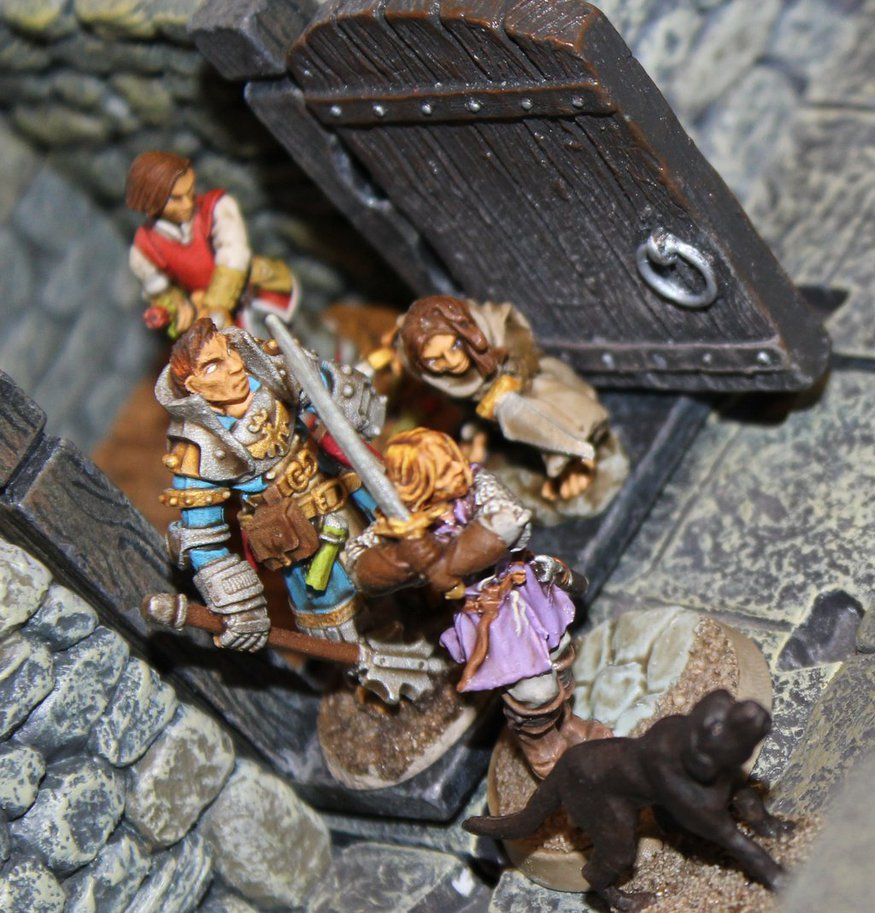
\includegraphics[width=3cm, height=4cm]{C:/privat/rpg/crimson_throne_book/latex/images/titlepage}};
	
		% \node[below right,font=\bfseries\setmainfont{Immortal}\large] (name) at (0,0) {PUK};
		% \node[below right] at (0, -0.45cm) {LN small human};
	
	% Init +0; Senses Perception +2
	% Languages Common
	% AC 11, touch 11, flat-footed 11
	% hp 5 (1HD)
	% Fort -1, Ref +0, Will +2
	% Speed 30 ft. (6 squares)
	% Melee dagger (small) +1 (1d3/19-20)
	% Ranged dagger (small/thrown) +1 (1d3/19-20)
	% Face 5 ft. Reach 5 ft.
	% Base Atk +0; CMB -1; CMD 9
	% Abilities Str 10, Dex 10, Con 8, Int 8, Wis 14, Cha 18
	
	
	
	\end{tikzpicture}
}
\end{center}

% \section{Test}
% \kant[1]